\documentclass[table, 12pt]{article}
\usepackage[a4paper, top=25mm, bottom=25mm, left=20mm, right=20mm]{geometry}
\usepackage{graphicx}
\usepackage[T1]{fontenc}
\usepackage[default]{cantarell}
\usepackage{tocloft}
\usepackage{caption}
\usepackage{minted}
\usepackage{hyperref}
\usepackage{booktabs}
\usepackage{listings}
\usepackage{pdfpages}
\usepackage{pdflscape}
\usepackage{textpos}
\usepackage{scrhack}
\usepackage{xcolor}
\usepackage{mathptmx}
\usepackage{float}
\usepackage{longtable}
\usepackage{enumitem}
\usepackage{tasks}
\usepackage{tabularx}
\usepackage{titlesec}
\usepackage{graphicx}
\usepackage {float}

\newcommand{\red}{\color{red}}

\titleformat{\paragraph}
{\normalfont\normalsize\bfseries}{\theparagraph}{1em}{}
\titlespacing*{\paragraph}
{0pt}{3.95ex plus 1ex minus .2ex}{.5ex plus .2ex}

\begin{document}
\setlength{\parindent}{0em}

\begin{titlepage}
    \centering
    \vspace{2cm}
    \scshape\large Academic Year 2020/2021 \par
    \vfill
    
\includegraphics[width=200pt]{images/LogoPoliMI}\par\vspace{1cm}
    {\scshape\LARGE Computer Science and Engineering \par}
    \vspace{1.5cm}
    {\Large\bfseries System and Methods for Big and Unstructured Data \par}
    \vspace{0.5cm}
    {\huge\bfseries \textbf{Project Report - MongoDB} \par}
    \vspace{2cm}
    {\large{Matteo Falzi - 10638723\\ Fabio La Manna - 10620549 \\ Filippo Manzardo - 10864201 \\ Paolo Marzolo - 10668259 \\ Matteo Regge -  10619213}\par}
    \vfill
    {\large Prof. Marco Brambilla }
    \vfill
    {\large \textbf{}\\ \today \par}
\end{titlepage}
\hypersetup{%
    pdfborder = {0 0 0}
}
\thispagestyle{plain}
\pagenumbering{gobble}
\mbox{}

%%%%%%%%%%%%%%%%%%%%%%%%%%%%%%%%%%%%%%%%%%%%%%%%%%%%%%%%%%%%%%%%%

\section{Introduction}

The measures taken by the Government for the management of the pandemic have generated a multitude of documents, the creation of an application for the management of these documents by the authorities and the citizen has become  far more than a need. The authorities  have created a Covid pass for people vaccinated and/ or tested. This pass removes the movement limits imposed by the restrictions due to the pandemic, allows access to bars, restaurants, cinemas, schools as it ensures that the citizen who is in possession of it is in a "safe" state of health, which implies it must be validated by the certified staff.


\subsection{Delivery specification}
The goal of the project is: designing, storing and using a documents NoSQL DB for collecting the personal information of the users and in addition their Covid tests, vaccination, Covid pass and the information of the authorized bodies that can deliver these certificates and using this information to support a certification app for COVID-19.. 





All the work done can be found at this link:
\href{https://github.com/pollomarzo/SAMBUD_proj2}{GitHub Repo}

\subsection{Assumptions}

\begin{description}
\item[Validation:] The certificate has two attributes for the validation, the version and the expiration date, for each version corresponds to a duration and consequently a different expiration date.
\item[Places:]We consider these places as the authorizing bodies (hospitals, pharmacies, clinics), they all have a name and geographic data.The dataset containing places was retrieved from \href{http://download.geonames.org/export/dump/}{GeoNames} and it has been pre-processed for better use. 
\item[Doctor/Nurse:] For each test/vaccine there are one doctor and at least one nurse ( max five nurses). 
 
\end{description} 
\newpage
%%%%%%%%%%%%%%%%%%%%%%%%%%%%%%%%%%%%%%%%%%%%%%%%%%%%%%%%%%%%%%%%%

\section{Relational Model}
To approach the problem, we developed an ER Model based of  7 entities: Person with Doctor and Nurse, Test, Vaccines,Place and the main certificate. 
Following the image of the ER diagram and the descriptions of the classes and relations.
\begin{figure}[H]
    \centering
    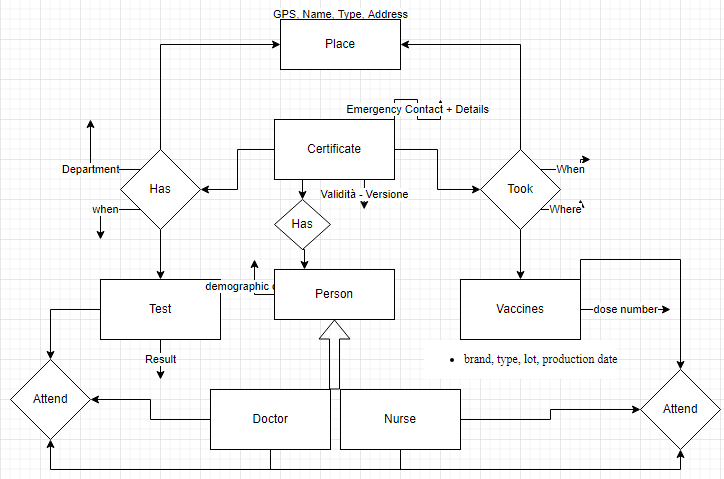
\includegraphics[width=\textwidth]{images/er.png}
    \caption{Entity-Relation Model}
    \label{fig:my_label}
\end{figure}
\subsection{Logical Model}
\begin{minted}
    [
    frame=lines,
    framesep=5mm,
    baselinestretch=1.5,
    escapeinside=||
    ]
    {python}
    ####### Entities #######
    Person(|\red{CIF}|,First_Name,Last_Name,Birth,Birthplace)
    Doctor(|\red{CIF}|,First_Name,Last_Name,Birth,Birthplace)
    Nurse(|\red{CIF}|,First_Name,Last_Name,Birth,Birthplace)
    Place(|\red{Code}|,Hospital_Unit,Lat,Long,CAP,Area,Area_name,NUTS1_Code,NUTS2_Code)
    Tests(|\red{CIF}|,|\red{Date}|,Results)
    Vaccines(|\red{CIF}|,|\red{Date}|,Brand,Type,Production_Date)
    Certificate(|\red{Code}|,Version,Expiration_date)
   
    
            
\end{minted}

\section{MongoDB Implementation}
To generate entities and relations, we coded a python script called "generate\_dataset.py", in the latest DB there are:
\begin{itemize}
    \setlength\itemsep{-0.5em}
    \item ~$9000$ Certificate \\
    \item ~$300$ Places \\
\end{itemize}
For a total of $38904$ nodes and $88110$ relations.
These numbers can be modified through the variables found in the first lines of the script. \\
Once that the script has been executed, 2 output json files can be found in scripts/output. 
\subsection{Queries}

Now we list some queries we wrote to inspect our database for useful information about COVID.

\subsubsection*{Query n. 1}
Count how many people have an expired certificate

\begin{minted}
    [
    frame=lines,
    framesep=5mm,
    baselinestretch=1.5,
    escapeinside=||
    ]
    {java}
db.Certificates.aggregate([
    { $match:{"Validity.Expiration_Date":{$lte:"2021-12-12" }}}, 
    { $count:"Expired_certificates" }
]) 

\end{minted}
\begin{figure}[H]
    \centering
    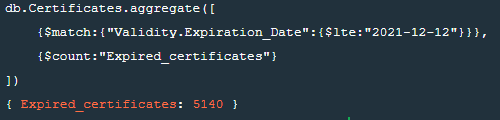
\includegraphics[width=\textwidth]{images/Q1.png}
\end{figure}
\subsubsection*{Query n. 2}
Count how many people did at least one mRna vaccine
\begin{minted}
    [
    frame=lines,
    framesep=5mm,
    baselinestretch=1.5,
    escapeinside=||
    ]
    {java}
    
db.Certificates.find(
    {Vaccines:{$elemMatch:{Type:"mRNA"}}}).count()
    
\end{minted}
\begin{figure}[H]
    \centering
    
\includegraphics[width=\textwidth]{images/Q2.png}
\end{figure}
\subsubsection*{Query n. 3}
Find the people who had two doses of Pfizer
\begin{minted}
    [
    frame=lines,
    framesep=5mm,
    baselinestretch=1.5,
    escapeinside=||
    ]
    {java}
    
db.Certificates.aggregate([
    {$project:{
                CIF:1, 
                Vaccines: {$filter:{input:"$Vaccines", as:"v", cond:{$eq:["$$v.Brand", "Pfizer"]}}}}}, 
    {$match:{"Vaccines" :{$size:2}}}
])

\end{minted}
\begin{figure}[H]
    \centering
    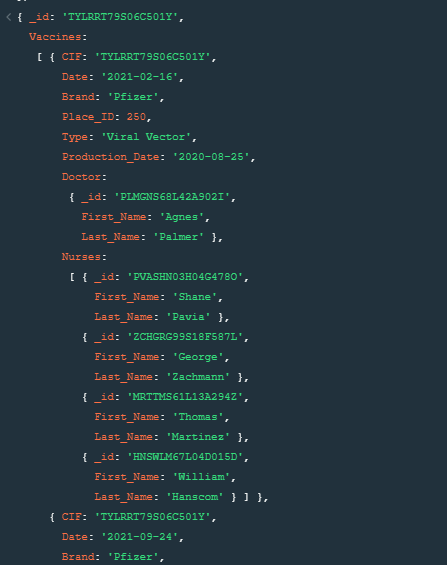
\includegraphics[width=\textwidth]{images/Q3.png}
\end{figure}
\newpage
\subsubsection*{Query n. 4}
Find the people who had a positive result in the last test they did
\begin{minted}
    [
    frame=lines,
    framesep=5mm,
    baselinestretch=1.5,
    escapeinside=||
    ]
    {java}
db.Certificates.aggregate([
     {$project:{
                _id:1, 
                Tests:{$reduce:{
                                input:"$Tests", 
                                initialValue:{Date:"0000-00-00"}, 
                                in:{$cond:[{$gte:["$$this.date", "$$value.date"]}, 
                                "$$this", "$$value"]}}}}}, 
     {$match:{"Tests.Result":true}}
])

\end{minted}
\begin{figure}[H]
    \centering
    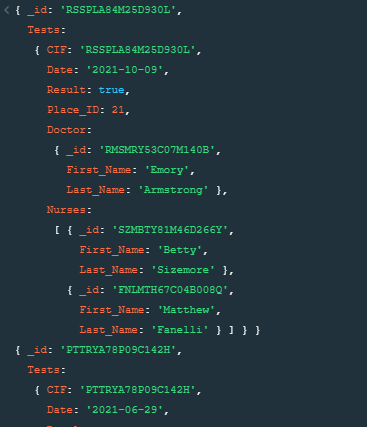
\includegraphics[width=\textwidth]{images/Q4.png}
\end{figure}
\subsubsection*{Query n. 5}
Find all the hospitals
\begin{minted}
 [
    frame=lines,
    framesep=5mm,
    baselinestretch=1.5,
    escapeinside=||
    ]
    {java}
db.Places.find({
      $text:{"$search":"Presidio Ospedaliero"}
}).limit(50)
\end{minted}
\begin{figure}[H]
    \centering
    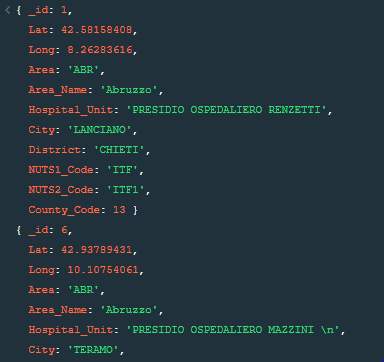
\includegraphics[width=\textwidth]{images/Q5.png}
\end{figure}
\subsubsection*{Query n. 6}
Find all the hospitals and order them with the text search score
\begin{minted}
 [
    frame=lines,
    framesep=5mm,
    baselinestretch=1.5,
    escapeinside=||
    ]
    {java}
db.Places.aggregate([
        {$match:{$text:{$search:"ospedale"}}}, {$sort:{score:{$meta:"textScore"}}}
])

\end{minted}
\begin{figure}[H]
    \centering
    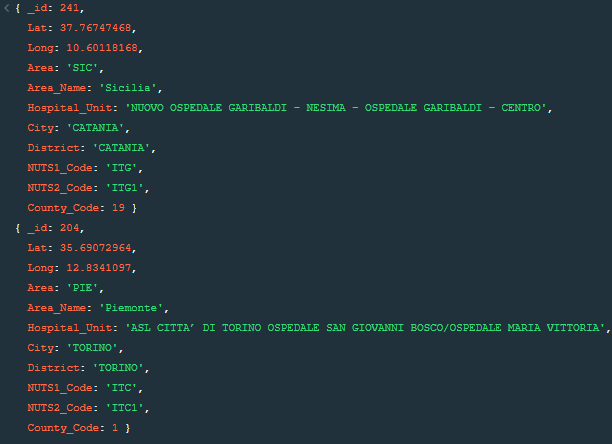
\includegraphics[width=\textwidth]{images/Q6.png}
\end{figure}

%%%%%%%%%%%%%%%%%%%%%%%%%%%%%%%%%%%%%%%%%%%%%%%%%%%%%%%%%%%%%%%%%

\newpage
\subsection{Commands}
Below some commands that manipulates the database. \\ 
(NOTE) The nodes generated with "generate\_dataset.py" are coerent with the assumptions, in order to get some corrupted CSV files, use "generate\_inconsistent\_dataset.py"
\subsubsection{Command n. 1}
For all certificates with version "v1", set the expiration date to: 31/12/2021
\begin{minted}
 [
    frame=lines,
    framesep=5mm,
    baselinestretch=1.5,
    escapeinside=||
    ]
    {java}
db.Certificates.updateMany(
      {"Validity.Version":"v1"}, 
      {$set:{"Expiration_Date":"2021-12-31"}}
)

\end{minted}
\begin{figure}[H]
    \centering
    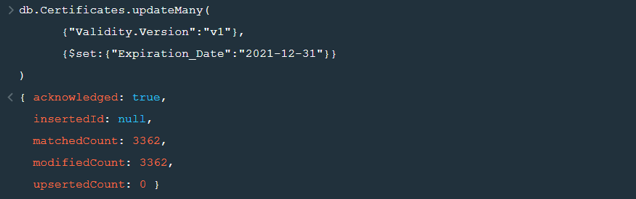
\includegraphics[width=\textwidth]{images/C1.png}
\end{figure}
\subsubsection{Command n. 2}
For all the people who did a vaccine in the place 168, set the doctor id to "null", doctor first name as "Flavio" and doctor last name as "Manna"

\begin{minted}
 [
    frame=lines,
    framesep=5mm,
    baselinestretch=1.5,
    escapeinside=||
    ]
    {java}
db.Certificates.updateMany(
      {"Vaccines.Place_ID":168}, 
      {$set:{"Vaccines.$.Doctor.0._id":"null", "Vaccines.$.Doctor.0.First_Name":"Flavio", "Vaccines.$.Doctor.0.Last_Name":"Manna"}}
)

\end{minted}
\begin{figure}[H]
    \centering
    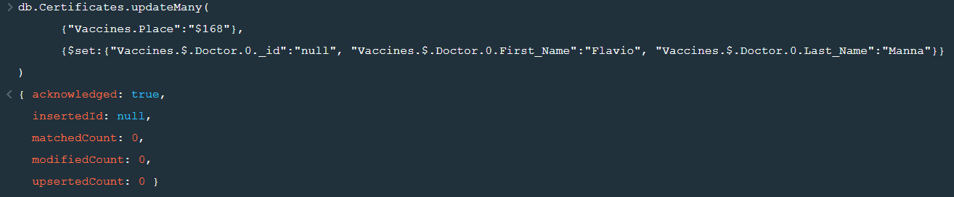
\includegraphics[width=\textwidth]{images/C22.png}
\end{figure}


\subsubsection{Command n. 3}
Delete all certificates without vaccine  
\begin{minted}
 [
    frame=lines,
    framesep=5mm,
    baselinestretch=1.5,
    escapeinside=||
    ]
    {java}
    
db.Certificates.deleteMany(
      {Vaccines:{$size:0}}
)

\end{minted}
\begin{figure}[H]
    \centering
    
\includegraphics[width=\textwidth]{images/C3.png}
\end{figure}



\section{User Interface Implementation}



%%%%%%%%%%%%%%%%%%%%%%%%%%%%%%%%%%%%%%%%%%%%%%%%%%%%%%%%%%%%%%%%%

\section{Conclusion and possible improvements}
In this report, we outlined the design and implementative choices behind the second part of the SAMBUD Fall 2021 project at Polimi.
The project highlights the potential of MongoDB, a documents based NoSQL DB,  as a modern way of storing and managing data compared to normal databases. From the practical point of view it has been  interesting  to see  how the complexity of the  ER model has become such a lean structure, highlighting the advantages of working on  documents. MongoDB allows for convenient data management, the queries were easy to understand and mirrored the underlying structure.
This project has broadened our understanding and vision of NoSQl DBc, using a storage structure that is inspired by the one of the real world allowing us to move away from the classic world of sql.

\end{document}

